\documentclass[border=10pt]{standalone}
\usepackage{xcolor}
\usepackage{pgfplots}
\usepackage{tikz}
\begin{document}
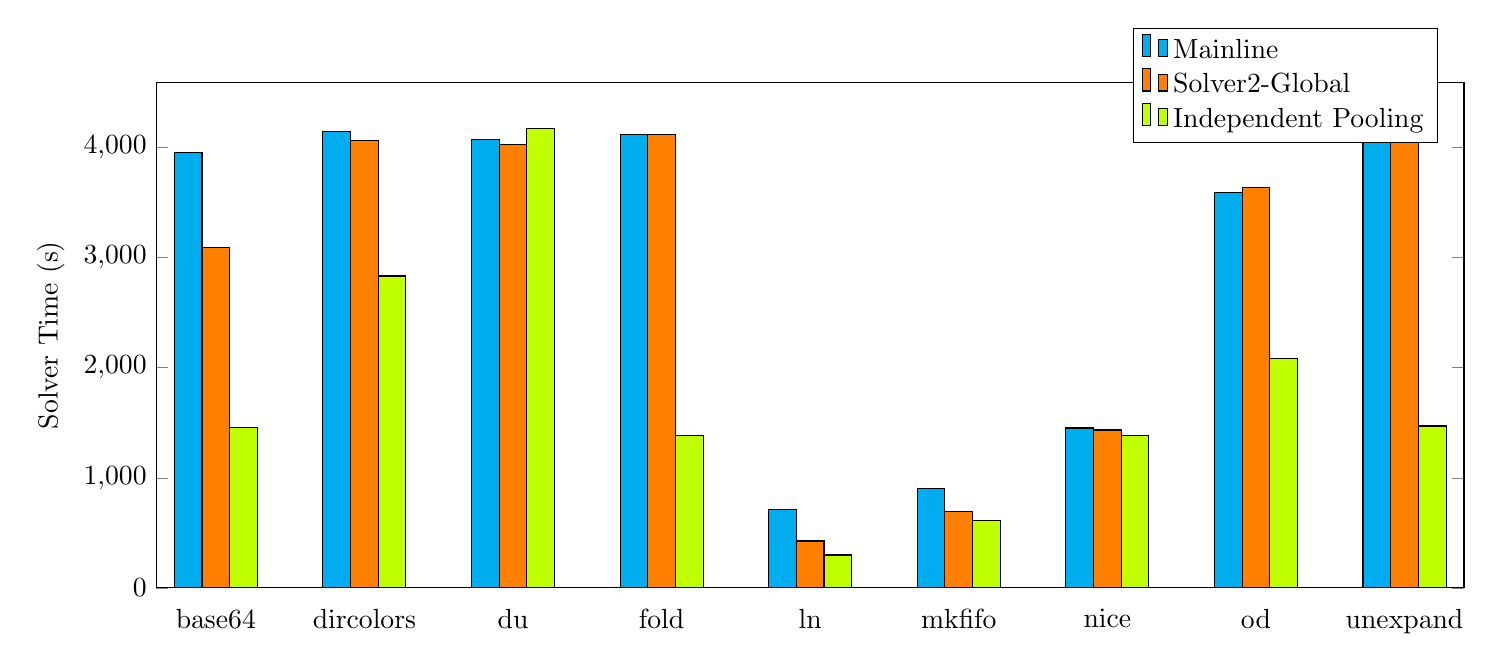
\begin{tikzpicture}
    \begin{axis}[
        width  = 1.5 * \textwidth,
        height = 8cm,
        major x tick style = transparent,
        % tickwidth=10,
        ybar=0,
        bar width=10pt,
        % ymajorgrids = true,
        ylabel = {Solver Time (s)},
        symbolic x coords={base64,dircolors,du,fold,ln,mkfifo,nice,od,unexpand},
        xtick = data,
        scaled y ticks = false,
        enlarge x limits=0.05,
        ymin=0,
        legend cell align=left,
        legend style={
                at={(0.98,0.88)},
                anchor=south east,
                % column sep=1ex
        }
    ]
        \addplot[style={cyan,fill=cyan,mark=none}, draw=black]
	coordinates {(base64,3951.19) (dircolors,4142.66) (du,4072.33) (fold,4120.91) (ln,715.61) (mkfifo,902.94) (nice,1452.47) (od,3591.29) (unexpand,4134.98)};
\addplot[style={orange,fill=orange,mark=none}, draw=black]
	coordinates {(base64,3094.59) (dircolors,4063.96) (du,4026.27) (fold,4114.99) (ln,425.56) (mkfifo,694.78) (nice,1433.72) (od,3633.46) (unexpand,4136.66)};
\addplot[style={lime,fill=lime,mark=none}, draw=black]
	coordinates {(base64,1458.20) (dircolors,2831.96) (du,4172.24) (fold,1381.37) (ln,299.10) (mkfifo,610.19) (nice,1382.92) (od,2085.38) (unexpand,1470.57)};

        \legend{Mainline,Solver2-Global,Independent Pooling}
    \end{axis}
\end{tikzpicture}
\end{document}
